\renewcommand{\thefootnote}{\arabic{footnote}}

\section{Data}

\begin{figure}[tb]
  \centerline{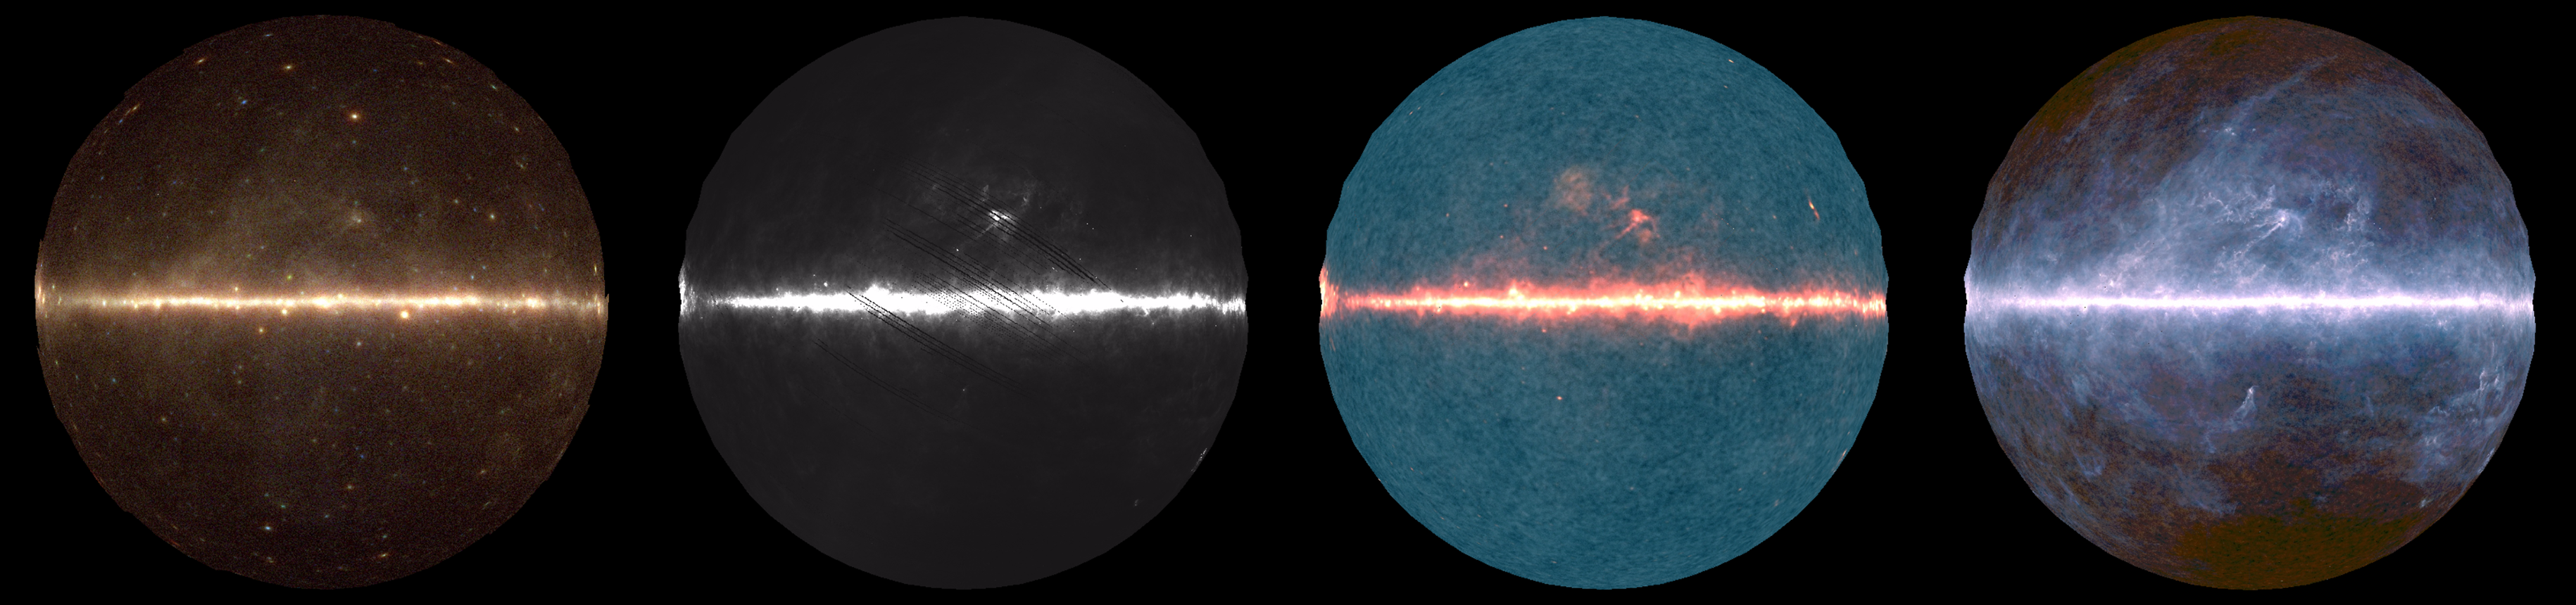
\includegraphics[width=\textwidth]{figures/four_images}}
  \caption{Survey images (left to right): Fermi color, AKARI 90um, Planck LFI, Planck HFI. Images centered on the Galactic Center, FOV 180 degrees.}
  \label{fig:four_images}
\end{figure}

\begin{figure}[tb]
  \centerline{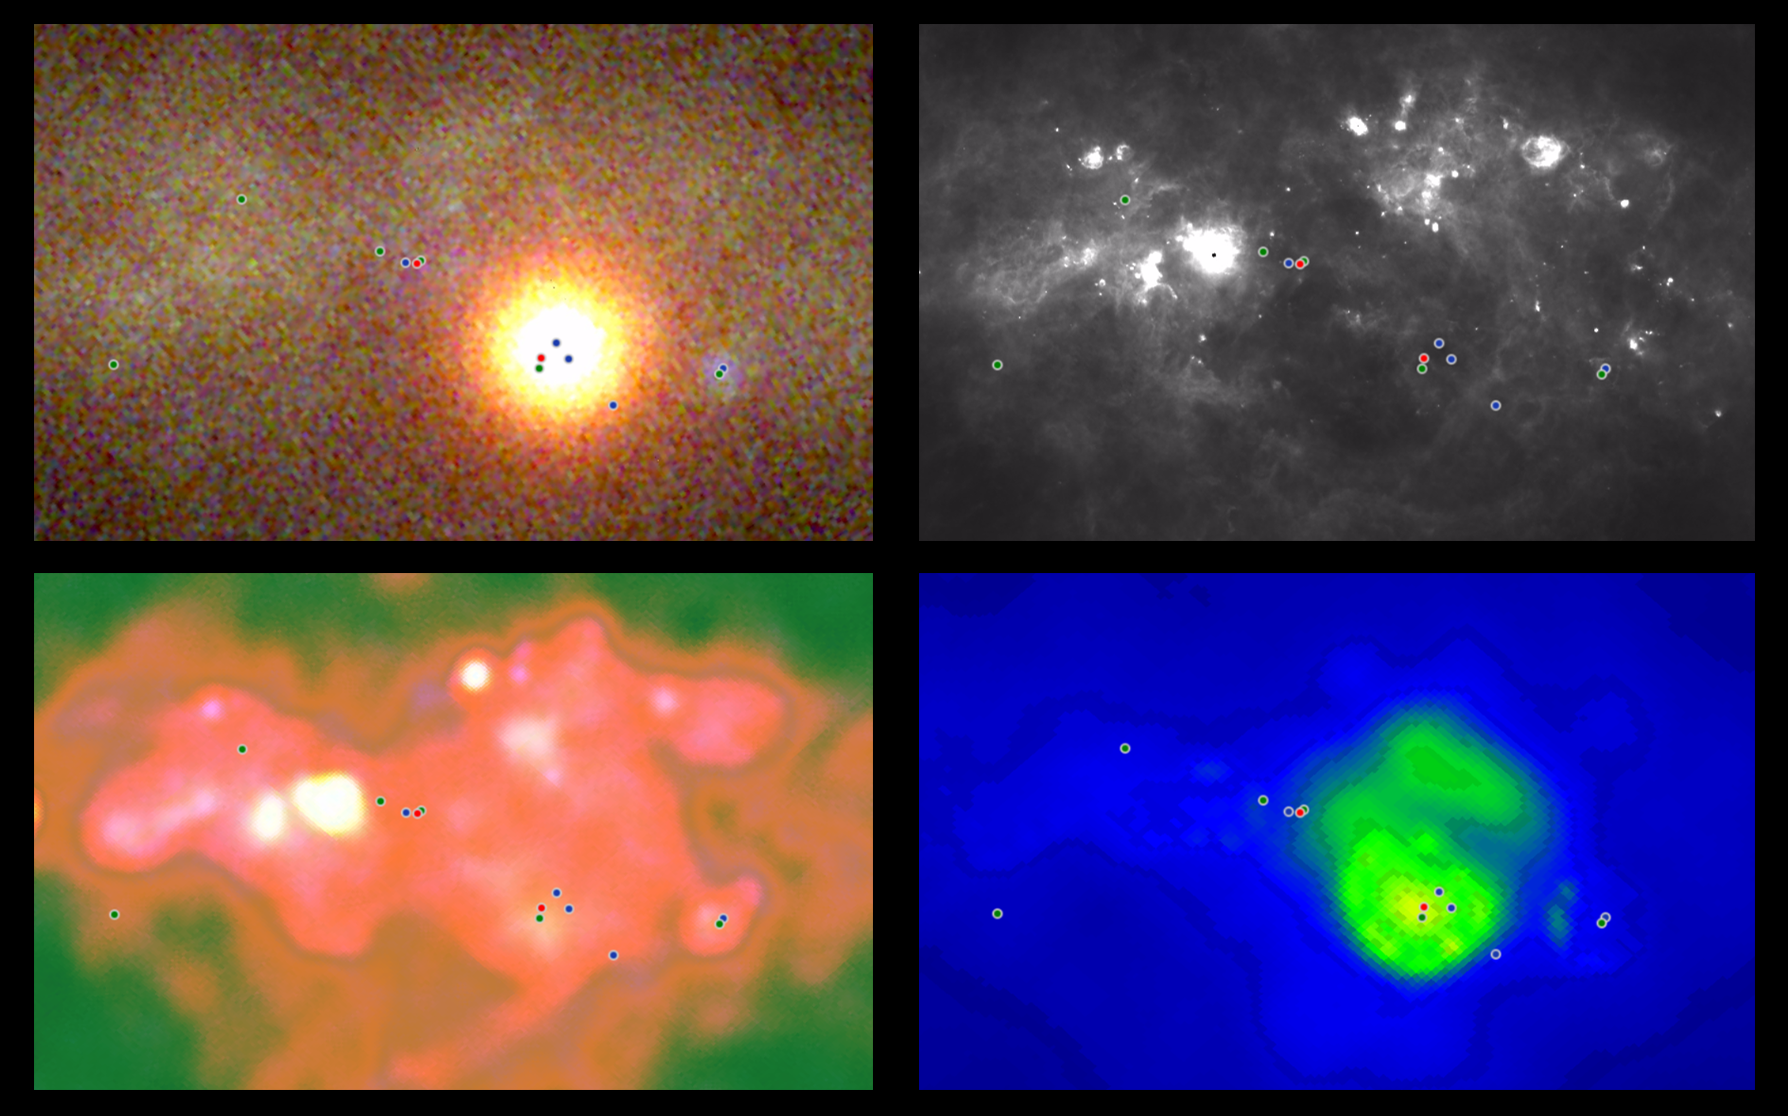
\includegraphics[width=\textwidth]{figures/vela_region}}
  \caption{The Vela Region in various survey images and color maps, FOV 20 degrees.}
  \label{fig:vela_region}
\end{figure}

% \begin{figure}[tb]
%   \centerline{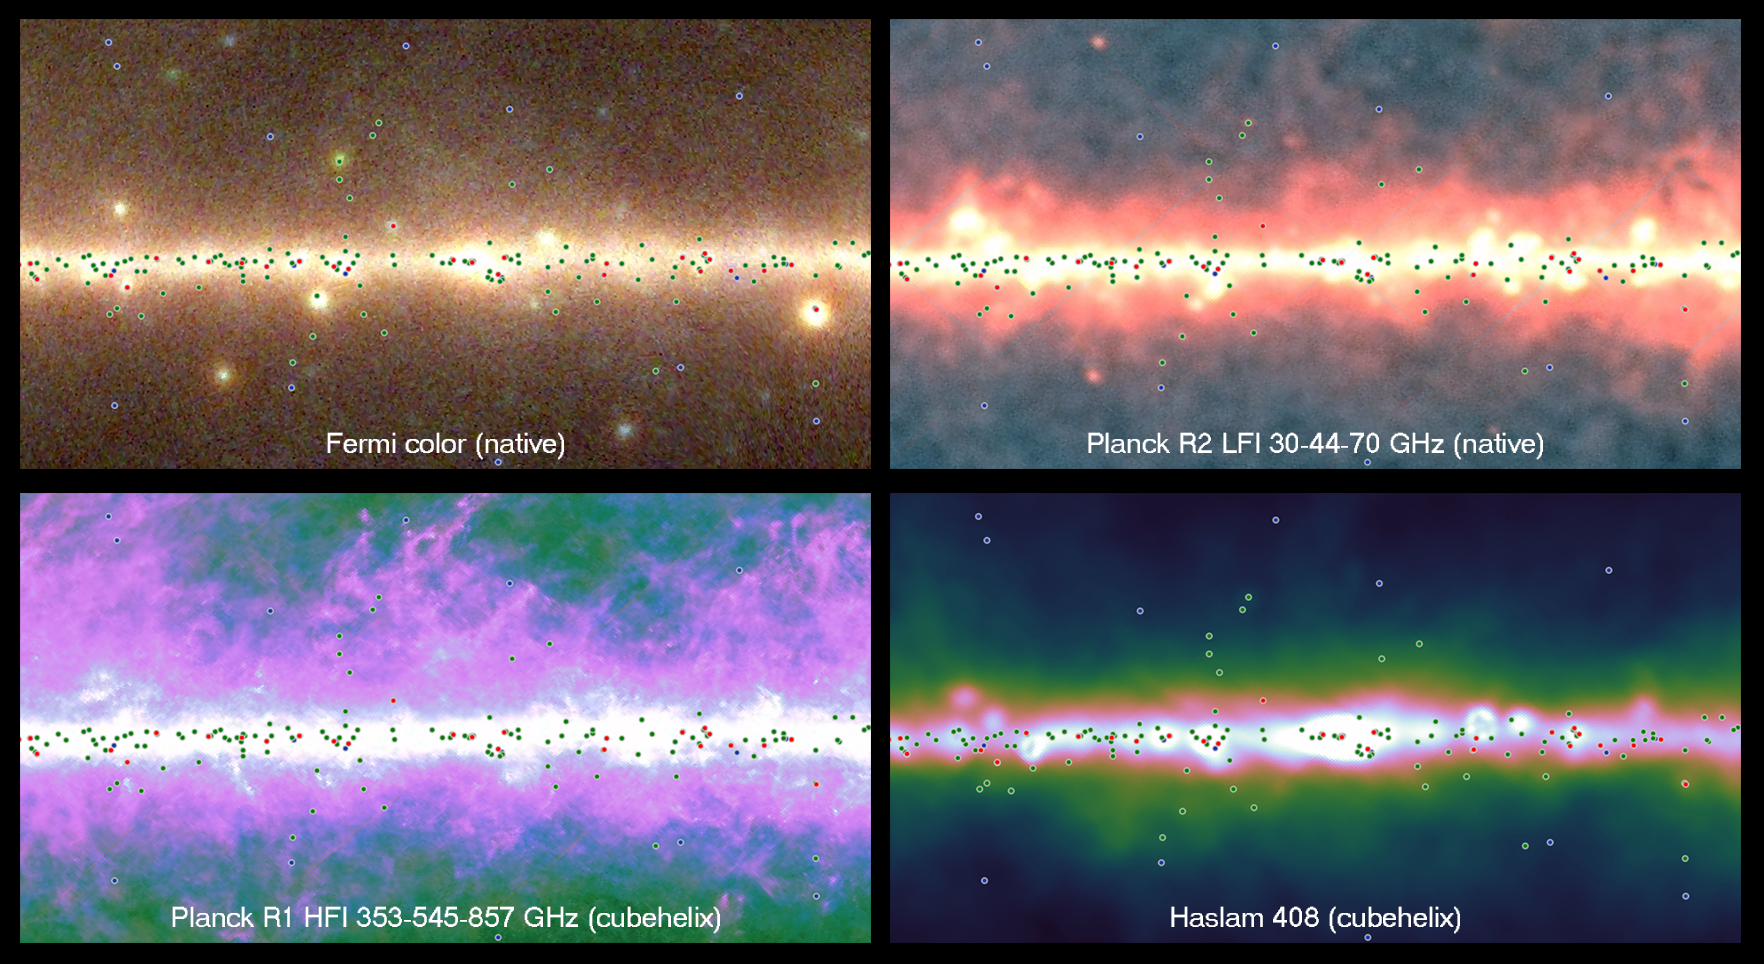
\includegraphics[width=\textwidth]{figures/inner_galaxy_region}}
%   \caption{The inner Galaxy in various survey images and color maps, FOV 45 degrees.}
% \end{figure}

% \begin{figure}[tb]
%   \centerline{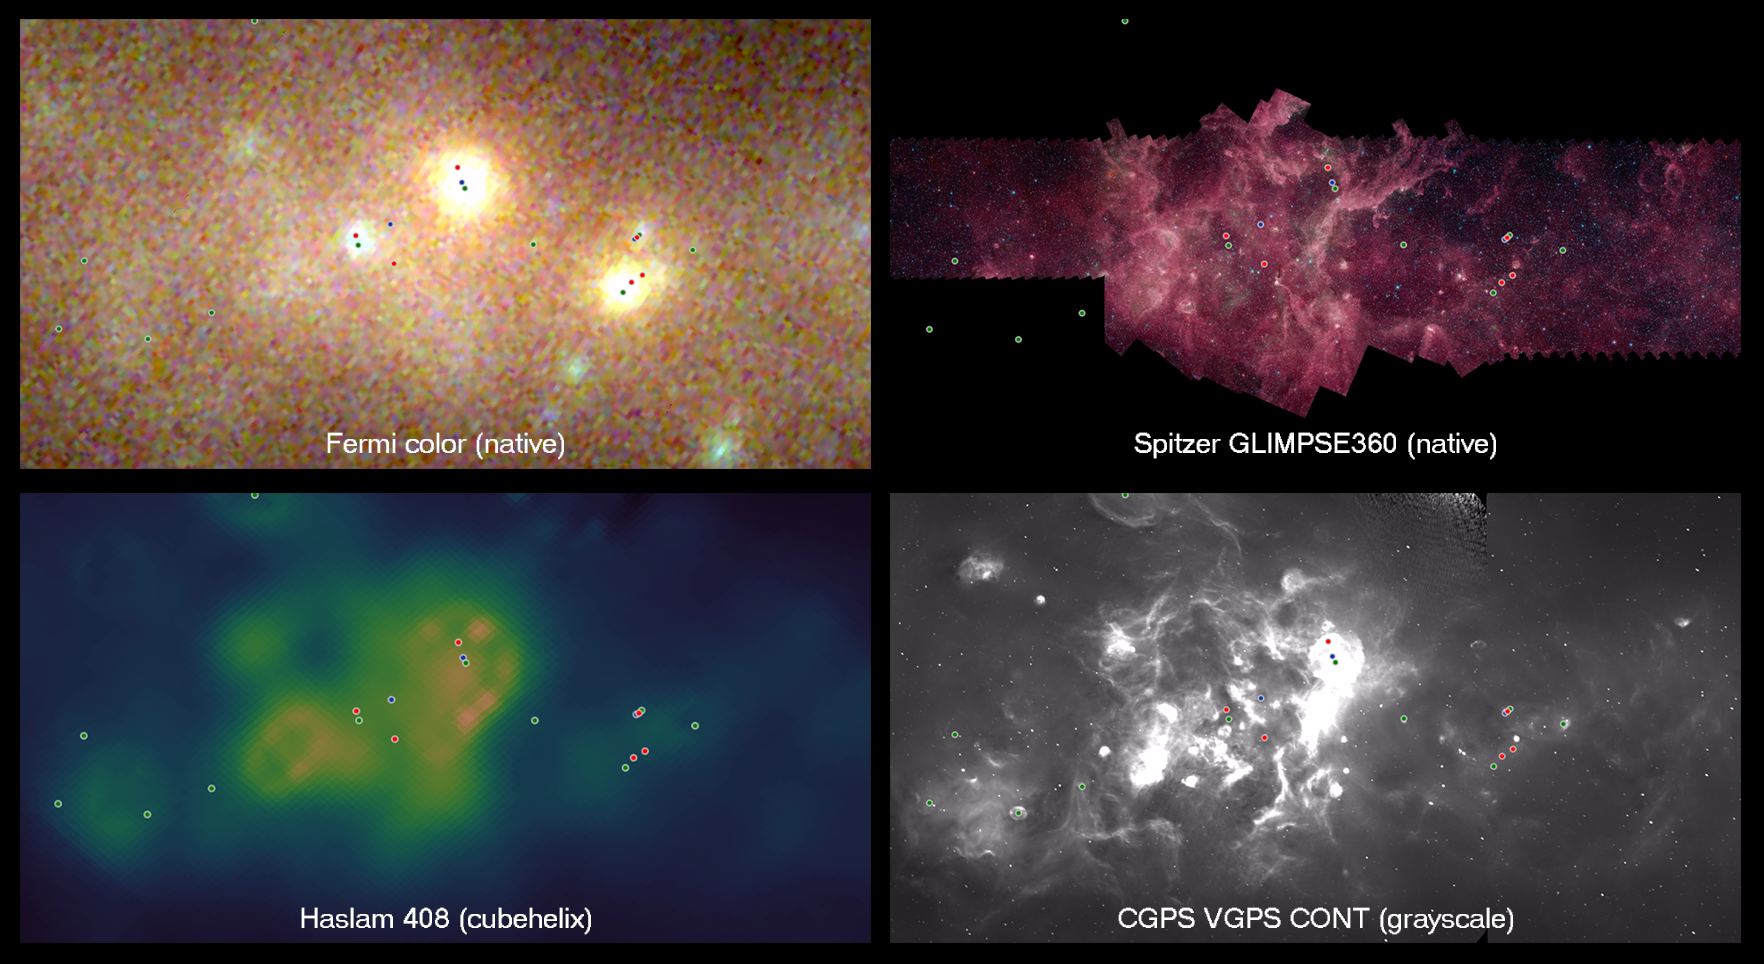
\includegraphics[width=\textwidth]{figures/cygnus_region}}
%   \caption{The Cygnus Region in various survey images and color maps, FOV 20 degrees.}
% \end{figure}

% \begin{figure}[tb]
%   \centerline{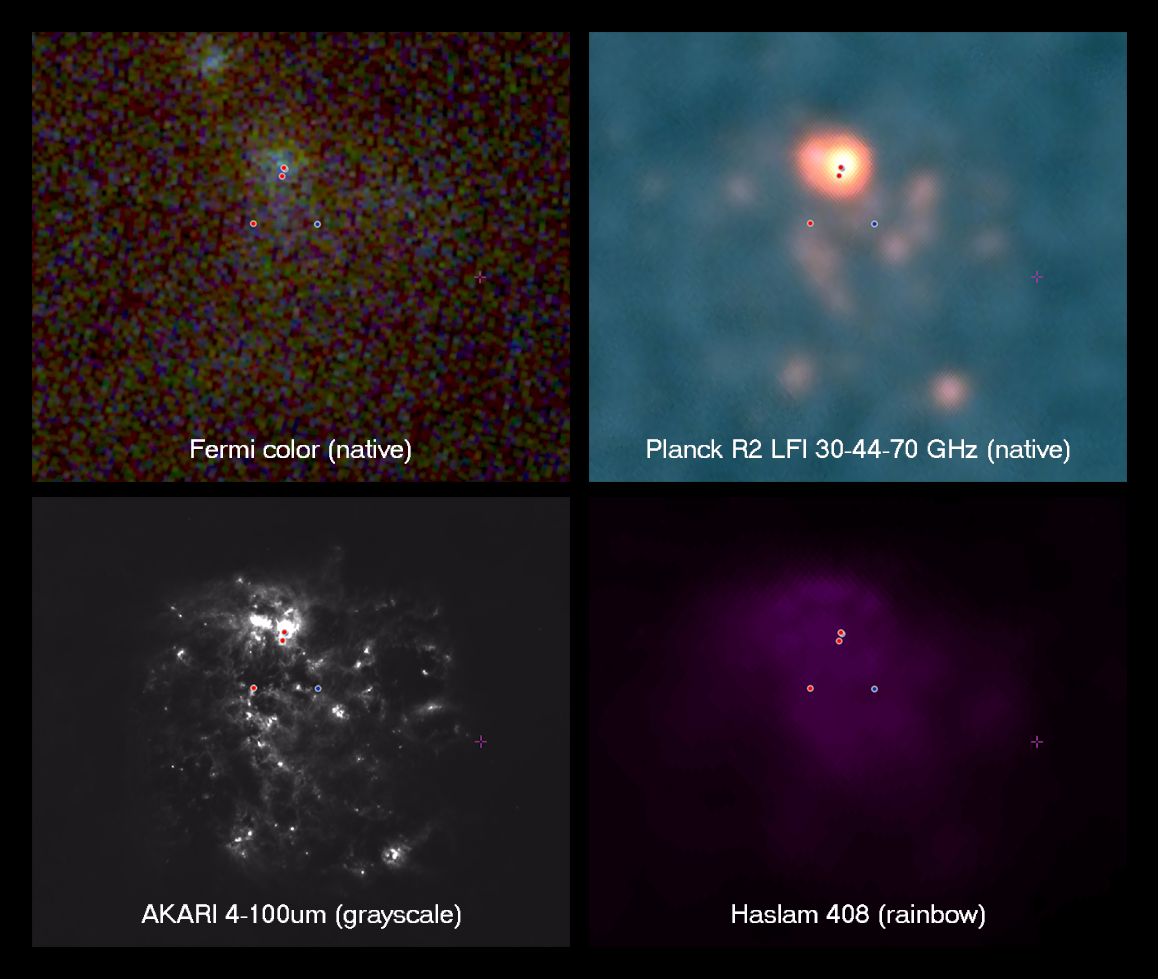
\includegraphics[width=\textwidth]{figures/lmc_region}}
%   \caption{The Large Magellanic Cloud (LMC) in various survey images and color maps, FOV 10 degrees.}
% \end{figure}

\begin{table}[bt]

\caption{
Survey images of interest to gamma-ray astronomers available on \gammasky . Note that this is only a very small selection, there are over 300 other multi-wavelength survey images available from CDS via Aladin Lite. The ones listed here were not produced by us specifically for \gammasky . We plan to add more gamma-ray survey images from the GeV energy range (high-energy Fermi-LAT data) and the TeV energy range (H.E.S.S. Galactic plane survey).
}
\label{tab:images}
\tabcolsep7pt\begin{tabular}{ lrlrl }
\hline
Image & Resolution (arcmin) & Type & Band & Coverage\\
\hline
Fermi-LAT & TBD & gamma-ray &  & all-sky\\
AKARI 90um & 1 & infrared &  & all-sky\\
CGPS-VGPS CONT & 1 & radio &  & galactic plane\\
Haslam 408 & 51 & radio & 408 MHz & all-sky\\
IRIS Band 4-100um & TBD & infrared &  & all-sky\\
Planck R1 + R2 HFI & TBD & microwave & 353-545-857 GHz & all-sky\\
Planck R2 LFI & TBD & microwave & 30-44-70 GHz & all-sky\\
Spitzer GLIMPSE360 & 0.02 & infrared &  & galactic plane\\
\multicolumn{5}{c}{300+ other HIPS survey images available from \url{http://aladin.u-strasbg.fr/hips/list}} \\
\hline
\end{tabular}

\end{table}


\begin{table}[bt]

\caption{
Source catalogs currently displayed on \gammasky .
We intend to add additional catalogs of interest to gamma-ray astronomers to the website in the future, including the upcoming H.E.S.S. and HAWC TeV source catalogs, as well as the ATNF Pulsar Catalogue.
}
\label{tab:catalogs}
\tabcolsep7pt\begin{tabular}{ lrll }
\hline
Catalog   & Sources & Updates    & Description \\
\hline
gamma-cat &     153 & continuous & Open TeV gamma-ray source catalog  \\
&&& \gammacat  \\
2FHL      &     360 & fixed      & Second Fermi-LAT catalog of high-energy sources \citep{2fhl}\\
&&& \url{http://fermi.gsfc.nasa.gov/ssc/data/access/lat/2FHL/}  \\
3FGL      &    3034 & fixed      & Third Fermi-LAT point source catalog \citep{3fgl}\\
&&& \url{http://fermi.gsfc.nasa.gov/ssc/data/access/lat/4yr_catalog/}  \\
SNRcat    &     378 & continuous & A census of high-energy observations of Galactic supernova remnants \citep{snrcat}\\
&&& \url{http://www.physics.umanitoba.ca/snr/SNRcat/} \\
\hline
\end{tabular}
\end{table}



The default base image layer displayed on gamma-sky.net's Map View page is a multi-wavelength all-sky survey from Fermi-LAT. In its native color map, source regions appear as certain colors according to their determined energies - red/yellow for 300-1000 MeV, green for 1-3 GeV, and blue for 3-300 GeV. The Fermi color image is presented on the website as a Heirarchical Progressive Survey (HiPS) image \cite{hips}. HiPS is a heirarchical data structure utilizing the HEALPix\footnote[1]{\url{http://healpix.sourceforge.net/}} tesselation of a sphere that organizes data onto pixelated tiles of scalable resolution. The image mechanism allows catalog data and source markers on gamma-sky.net to be visualized accurately on the sky map at various zoom levels. The Centre de Donn\'{e}es astronomiques de Strasbourg (CDS) developed the HiPS technology, and gamma-sky.net currently encompasses 8 survey images also prepared by CDS in this format. The 8 images, which are outlined in Table~\ref{tab:images}, come from CDS's HiPS database\footnote[2]{\url{http://aladin.u-strasbg.fr/hips/list}}, of over 300 prepared HiPS images.

Our website incorporates 4 catalogs which are displayed in Table~\ref{tab:catalogs}. 3FGL \cite{3fgl} and 2FHL \cite{2fhl} are the latest surveys from Fermi-LAT, the main space-based instrument we display sources from. SNRcat \cite{snrcat} is an up-to-date compilation of galactic SNRs observed from a variety of instruments. The database is maintained by the University of Manitoba and can be accessed at \url{http://www.physics.umanitoba.ca/snr/SNRcat/}. gamma-cat is an open-data catalog of sources in the TeV range. As a project that has just recently begun in early September 2016, it is undergrowing rapid growth and will be updated frequently on gamma-sky.net. gamma-cat was started at the Max-Planck-Institut f\'{u}r Kernphysik (MPIK) and is open to contribution from other developers. All of its catalog information can be found at \url{https://gammapy.github.io/gamma-cat/}.

User inputs for search fields under the Map View portion of the website are interpreted by the Sesame service\footnote[3]{\url{http://cds.u-strasbg.fr/cgi-bin/Sesame}}. Sesame is a search term resolver for astronomical objects which queries several databases and returns the resolved sources. Both Sesame and the databases searched (Simbad, NED, and VizieR) are maintained by CDS.

Under the Catalog View of gamma-sky.net, we are currently showing 3FGL light curve and emission spectrum plots from NASA's Fermi-LAT 3FGL Catalog Interactive Table\footnote[4]{\url{http://fermi.gsfc.nasa.gov/ssc/data/access/lat/4yr_catalog/3FGL-table}}.

TODO: Fix table + image placement after all other text is finalized.

TODO: For the image table (Table 2), we need to fill in the rest of the Band column (or remove the column alltogether)
